%\input{preamble.txt}
%
%\begin{document}
\section{SOLID Design}

\begin{itemize}
	\item What is SOLID?
	\begin{itemize}
		\item \textbf{S}ingle Responsibility Principle
		\item \textbf{O}pen/Closed Principle
		\item \textbf{L}iskov Substitution Principle
		\item \textbf{I}nterface Segregation Principle
		\item \textbf{D}ependency Inversion Principle
	\end{itemize}

	\item Single Responsibility Principle (SRP)\\
	\textbf{\emph{A class should have only one reason to change}}
	\begin{itemize}
		\item If you can think of more than one motive for changing a class, then that class has more than one responsibility
		\item If a class has more than one responsibility, then the responsibilities become coupled
		\item Violating the SRP\\
		\begin{center}
			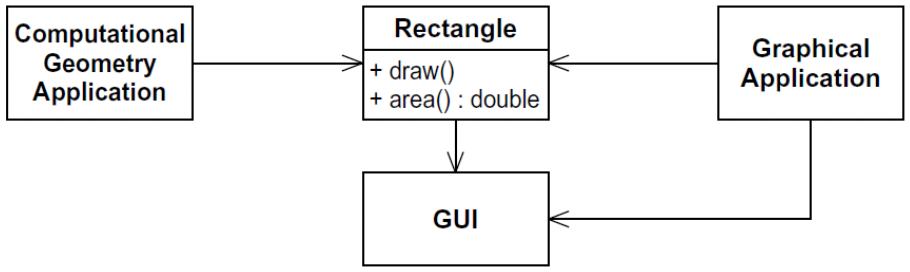
\includegraphics[width=0.6\linewidth]{SRPViolation}
		\end{center}
		\item Conforming to the SRP
		\begin{center}
			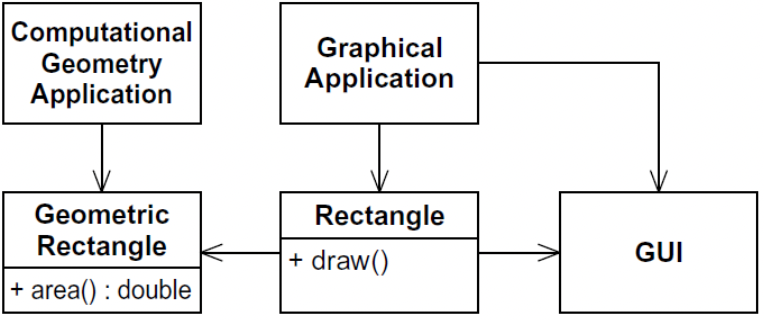
\includegraphics[width=0.5\linewidth]{SRPConform}
		\end{center}
	\end{itemize}

	\item The Open/Closed Principle (OCP)\\
	\textbf{\emph{Software entities (classes, modules, functions, etc.) should be open for extension, but closed for modification.}}
	\begin{itemize}
		\item When a single change to a program results in a cascade of changes to dependent modules, the design smells of rigidity.
		\begin{itemize}
			\item If the Open/Closed principle is applied well, then further changes of that kind are achieved by adding new code, not by changing old code that already works.
		\end{itemize}
		\item In Java, it is possible to create abstractions that are fixed and yet represent an unbounded group of possible behaviors
		\begin{itemize}
			\item The abstractions are abstract base classes, and the unbounded group of possible behaviors is represented by all the possible derivative classes.
		\end{itemize}
		\item Violating the OCP
		\begin{itemize}
			\begin{minipage}{0.5\textwidth}
				\item Both classes are concrete
				\item The \textbf{Client} uses the \textbf{Server} class
			\end{minipage}
			\begin{minipage}{0.5\textwidth}
				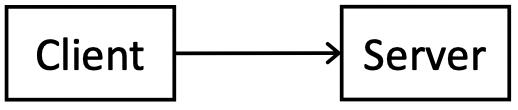
\includegraphics[width=1.5in]{OCPViolate}
			\end{minipage}
		\end{itemize}

		\begin{minipage}{0.5\textwidth}
			\item Conforming to the OCP\\
		\end{minipage}
		\begin{minipage}{0.5\textwidth}
			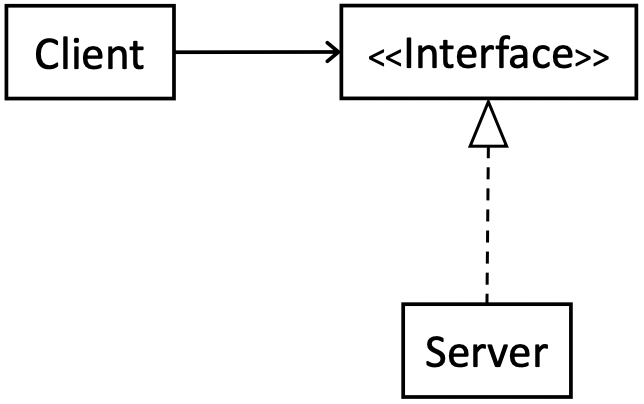
\includegraphics[width=0.4\textwidth]{OCPConform}
		\end{minipage}
	\end{itemize}

	\item The Liskov Substitution Principle (LSP)\\
	\textbf{\emph{Subtypes must be substitutable for their base types.}}
	\begin{itemize}
		\item Formally: Let $ \Phi(x) $ be a property provable about objects $ x $ of type $ T $. Then $ \Phi(y) $ should be true for objects $ y $ of type $ S $ where $ S $ is a subtype of $ T $.
		\item Counter-example: ``If it looks like a duck, quacks like a duck, but needs batteries – you probably have the wrong abstraction"
		\item Violating the LSP\\
		Issues:\\
		\begin{minipage}{0.6\textwidth}
			\begin{itemize}
				\item Inheriting \textbf{height} and \textbf{width}
				\item Overriding \textbf{setHeight} and \textbf{setWidth}
				\item Conflicting assumptions. For example:
				\begin{Verbatim}
	void testRectangleArea(Rectangle r){
		r.setWidth(5);
		r.setHeight(4);
		assertEquals(r.computeArea(), 20);
	}
				\end{Verbatim}
			\end{itemize}
		\end{minipage}
		\begin{minipage}{0.3\textwidth}
			\hspace*{2cm}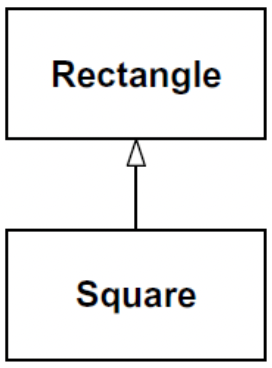
\includegraphics[width=1in]{LSPExample}
		\end{minipage}

		\item Implication: A model, viewed in isolation, cannot be meaningfully validated.
		\begin{itemize}
			\item The validity of a model can only be expressed in terms of its clients.
			\item One must view the design in terms of the reasonable assumptions made by
			the users of that design.
		\end{itemize}
	\end{itemize}

	\item The Interface Segregation Principle (ISP)\\
	\textbf{\emph{Clients should not be forced to depend on methods that they do not use.}}
	\begin{itemize}
		\item This principle deals with classes whose interfaces are not cohesive. That is, the interfaces of the class can be broken up into groups of methods where each group serves a different set of clients.
		\item When clients are forced to depend on methods that they don’t use, then those clients are subject to changes to those methods.\\
		\begin{minipage}[t]{0.4\textwidth}
			\item Violating the ISP\\
			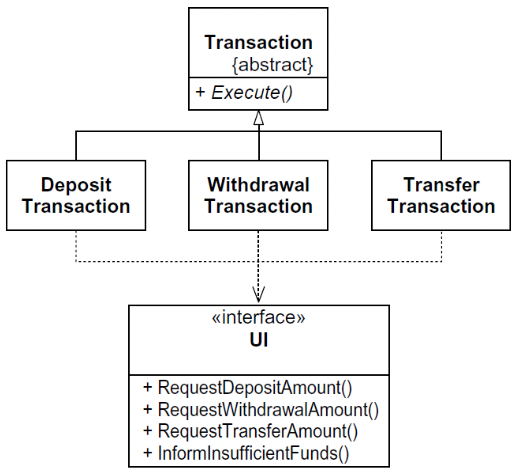
\includegraphics[width=2.5in]{ISPViolation}
		\end{minipage}
		\begin{minipage}[t]{0.6\textwidth}
			\item Conforming to the ISP\\
			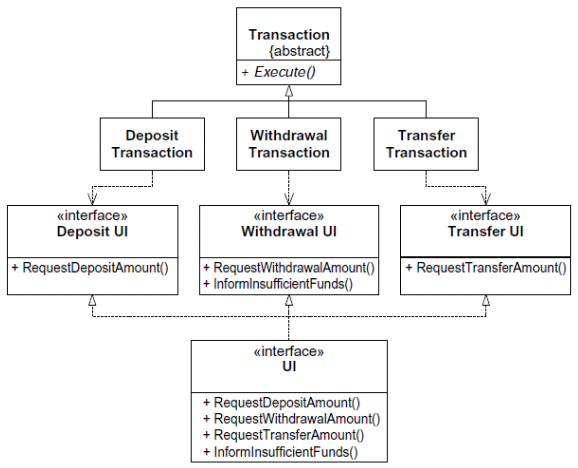
\includegraphics[width=3.5in]{ISPObey}
		\end{minipage}
	\end{itemize}

	\newpage

	\item The Dependency-Inversion Principle (DIP)
	\begin{enumerate}
		\item[\textbf{\textit{A.}}]  \textbf{\textit{High-level modules should not depend on low-level modules. Both should depend on abstractions.}}
		\item[\textbf{\textit{B.}}] \textbf{\textit{Abstractions should not depend on details. Details should depend on abstractions.}}
	\end{enumerate}
	\begin{itemize}
		\item The modules that contain the high-level business rules should take precedence over, and be independent of, the modules that contain the implementation details.
		\item When high-level modules depend on low-level modules, it becomes very difficult to reuse those high-level modules in different contexts.\\
		\begin{minipage}[t]{0.3\textwidth}
			\begin{center}
				\underline{\textbf{Naïve Layering}}\\
				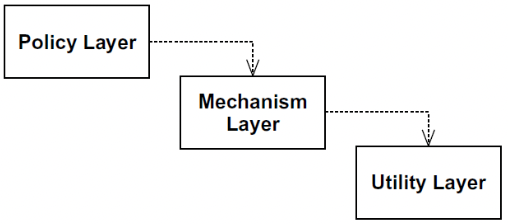
\includegraphics[width=2in]{DIPNaive}
			\end{center}
		\end{minipage}
		\begin{minipage}[t]{0.5\textwidth}
			\begin{center}
				\underline{\textbf{Inverted Layers}}\\
				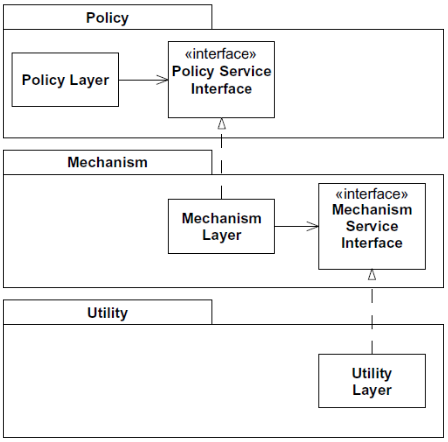
\includegraphics[width=2.5in]{DIPInverted}
			\end{center}
		\end{minipage}
		\\[10pt]
		\begin{minipage}[t]{0.5\textwidth}
			\item Violating the DIP\\
			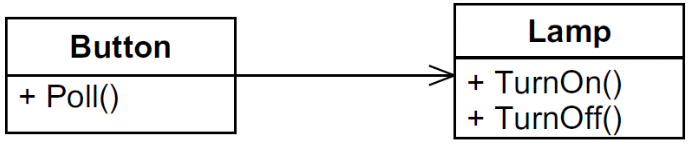
\includegraphics[width=2in]{DIPViolate}
		\end{minipage}
		\begin{minipage}[t]{0.5\textwidth}
			\item Conforming to the DIP\\
			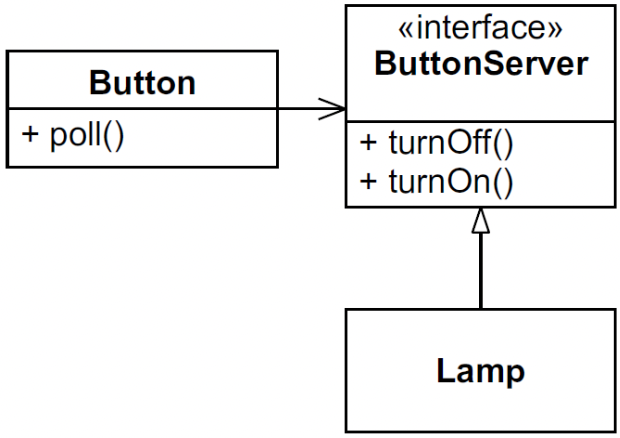
\includegraphics[width=2in]{DIPConform}
		\end{minipage}
	\end{itemize}

	\item Design Smells
	\begin{itemize}
		\item Symptoms of poor design
		\item Often caused by the violation of one or more of the design principles
		\begin{itemize}
			\item For example, the smell of \textit{Rigidity} is often a result of insufficient attention to OCP.
		\end{itemize}
		\item These symptoms include:
		\begin{enumerate}
			\item Rigidity -- The design is hard to change.
			\item Fragility -- The design is easy to break.
			\item Immobility -- The design is hard to reuse.
			\item Viscosity -- It is hard to do the right thing.
			\item Needless Complexity -- Overdesign.
			\item Needless Repetition -- Mouse abuse.
			\item Opacity -- Disorganized expression.
		\end{enumerate}
	\end{itemize}
\end{itemize}

%\end{document}